\begin{frame}{Introduction to Coding Theory}

    \begin{columns}
        \begin{column}{0.5\textwidth}
            \begin{itemize}
  
                \item \uncover<1->{In 1948 Shannon published "A Mathematical Theory of Communication".}
                \uncover<2->{ \item In 1949 the Binary Goolay Codes where developed, capable of correcting up to 3 errors in a 24 bit string.}
                \uncover<3->{\item In 1959 Hamming develops the Hamming codes} \uncover<4->{ out of frustration:} \uncover<5->{\\ \hspace{1cm}"Damn it, if the machine can detect an error, why can't it locate the position of the error and correct it?"}
            \end{itemize}
        \end{column}
        \begin{column}{0.5\textwidth}
           \uncover<3->{ \includegraphics[width=0.7\textwidth]{Richard_Hamming.jpg}}
        \end{column}
    \end{columns}
\end{frame}

\begin{frame}

    \vspace{-2cm} % Adjust the vertical space as needed
    \hspace{2.3cm}\textcolor{red}{How?} \pause 
    \begin{center}
        \alert<1>{\Huge Redundancy!} \\ \pause
    \end{center}
    \pause
    Let's repeat each row of a message three times and then send it.\\ \pause
    If we obtain the message:
    \pause
    \only<5>{
    \begin{center}
         \begin{tabular}{|c|c|c|c|c|c|c|c|c|}
        \hline
        0 & 0 & 0 & 1 & 0 & 1 & 0 & 0 & 0 \\
        \hline
        0 & 0 & 0 & 1 & 1 & 1 & 0 & 0 & 0 \\
        \hline
        0 & 0 & 0 & 1 & 1 & 1 & 0 & 0 & 0 \\
        \hline
        \end{tabular}
    \end{center}
    }
    
    \uncover<6->{
    \begin{center}
         \begin{tabular}{|c|c|c|c|c|c|c|c|c|}
        \hline
        0 & 0 & 0 & 1 & \cellcolor{red!20}0 & 1 & 0 & 0 & 0 \\
        \hline
        0 & 0 & 0 & 1 & \cellcolor{red!20} 1 & 1 & 0 & 0 & 0 \\
        \hline
        0 & 0 & 0 & 1 & \cellcolor{red!20} 1 & 1 & 0 & 0 & 0 \\
        \hline
        \end{tabular}
            
    \end{center}
    }
    \pause
    \bigskip
    
    Since "1" appears twice and "0" once, we may assume more likely that the original message was:
    \pause
    \bigskip
    
    \begin{center}
    \begin{tabular}{|c|c|c|c|c|c|c|c|c|}
        \hline
        0 & 0 & 0 & 1 & \cellcolor{green!20} 1 & 1 & 0 & 0 & 0 \\
        \hline
    \end{tabular}
    \end{center}
    \pause
    \bigskip
    
    But this way, we took three times the length of the message to correct one error!
    
    \bigskip
    \pause
    \textcolor{gray}{Btw the message says SOS in Morse, so maybe go seek help.}
    \end{frame}
    
\begin{frame}{A better way to do it}
We rearrange the original message
\begin{tabular}{|c|c|c|c|c|c|c|c|c|}
    \hline
    \rowcolor{blue!20} 0 & 0 & 0 & 1 &  1 & 1 & 0 & 0 & 0 \\
    \hline
\end{tabular}
in a 4 by 4 grid: \\ 
\begin{center}
\pause
\begin{tabular}{|c|c|c|c|}
\hline
     &  \cellcolor{red!20} 0 & \cellcolor{red!20} 0 & \cellcolor{blue!20}  0  \\ \hline
    \cellcolor{red!20} 1 & \cellcolor{blue!20} 0 & \cellcolor{blue!20}  0 & \cellcolor{blue!20} 1  \\ \hline
    \cellcolor{red!20} 0 & \cellcolor{blue!20} 1 &\cellcolor{blue!20}  1 &\cellcolor{blue!20} 0  \\ \hline
    \rowcolor{blue!20}0 & 0 & 0 & 0  \\ \hline
\end{tabular}
\end{center}
\pause
Where the red cells are the four redundant bits which encode the parity of subsets of columns or rows in the following way. \\
\pause
\only<4>{   
\begin{minipage}{0.4\textwidth}
        \begin{center}
    \begin{tabular}{|c|c|c|c|}
        \hline
          &  \cellcolor{red!35} 0 & 0 & \cellcolor{blue!20}  0  \\ \hline
        1 & \cellcolor{blue!20} 0 &  0 & \cellcolor{blue!40} 1  \\ \hline
        0 & \cellcolor{blue!40} 1 &  1 &\cellcolor{blue!20} 0  \\ \hline
        0 & \cellcolor{blue!20} 0 & 0 &  \cellcolor{blue!20} 0  \\ \hline
\end{tabular}
\end{center}
\end{minipage}
%
\begin{minipage}{0.4 \textwidth}
    \begin{center}
        \cell{0}{red!35} = \cell{1}{blue!40} + \cell{1}{blue!40}
    \end{center}
\end{minipage}
}
\only<5>{   
\begin{minipage}{0.4\textwidth}
        \begin{center}
    \begin{tabular}{|c|c|>{\columncolor{blue!20}}c|>{\columncolor{blue!20}}c|c|} 
    \hline
          &  0 & \cellcolor{red!30}0  &  0  \\ \hline
        1 & 0 &  0 & \cellcolor{blue!40}1  \\ \hline
        0 & 1 &  \cellcolor{blue!40}1 & 0  \\ \hline
        0 & 0 & 0 &  0  \\ \hline
\end{tabular}
\end{center}
\end{minipage}
%
\begin{minipage}{0.4 \textwidth}
    \begin{center}
        \cell{0}{red!35} = \cell{1}{blue!40} + \cell{1}{blue!40}
    \end{center}
\end{minipage}
}
\only<6>{   
\begin{minipage}{0.4\textwidth}
        \begin{center}
    \begin{tabular}{|c|c|c|c|}
        \hline
          &  0 & 0 &  0  \\ \hline
        \rowcolor{blue!20} \cellcolor{red!30}1 & 0 &  0 & \cellcolor{blue!40}1  \\ \hline
        0 & 1 &  1 & 0  \\ \hline
        \rowcolor{blue!20} 0 & 0 & 0 &  0  \\ \hline
\end{tabular}
\end{center}
\end{minipage}
%
\begin{minipage}{0.4 \textwidth}
    \begin{center}
        \cell{1}{red!35} = \cell{1}{blue!40} 
    \end{center}
\end{minipage}
}
\uncover<7->{
\begin{minipage}{0.4\textwidth}
        \begin{center}
    \begin{tabular}{|c|c|c|c|}
        \hline
          &  0 & 0 &  0  \\ \hline
        1 & 0 &  0 & 1  \\ \hline
        \rowcolor{blue!20} \cellcolor{red!35}0 & \cellcolor{blue!40} 1 &  \cellcolor{blue!40} 1 & 0  \\ \hline
        \rowcolor{blue!20} 0 & 0 & 0 &  0  \\ \hline
\end{tabular}
\end{center}
\end{minipage}
%
\begin{minipage}{0.4 \textwidth}
    \begin{center}
        \cell{0}{red!35} = \cell{1}{blue!40} + \cell{1}{blue!40}
    \end{center}
\end{minipage}
}
\hfill \\
\bigskip
\pause
\uncover<8->{
Since \(2^4 = \text{total number of bits} + (\text{case in which there is no error}) = 15 + 1\) and if there is up to one error, every redundant bit halvens the number the possible locations of where the error might be, we can always correct up to one error in the message.}
\end{frame}


\begin{frame}

    \only<1>{
        \begin{minipage}{0.4\textwidth}
            \begin{center}
        \begin{tabular}{|c|c|c|c|c|} 
        \hline
              &  0 & 0  &  1  \\ \hline
            1 & 0 &  0 & 1  \\ \hline
            0 & 1 &  1 & 0  \\ \hline
            0 & 0 & 0 &  0  \\ \hline
    \end{tabular}
    \end{center}
    \end{minipage}
    }
    \only<2>{
        \begin{minipage}{0.4\textwidth}
            \begin{center}
        \begin{tabular}{|c|c|c|c|c|} 
        \hline
              &  0 & \cellcolor{red!30}0  &  1  \\ \hline
            1 & 0 &  0 &1  \\ \hline
            0 & 1 &  1 & 0  \\ \hline
            0 & 0 & 0 &  0  \\ \hline
    \end{tabular}
    \end{center}
    \end{minipage}
    }
    \only<3>{
        \begin{minipage}{0.4\textwidth}
            \begin{center}
        \begin{tabular}{|c|c|>{\columncolor{blue!20}}c|>{\columncolor{blue!20}}c|c|} 
        \hline
              &  0 & \cellcolor{red!30}0  &  1  \\ \hline
            1 & 0 &  0 &1  \\ \hline
            0 & 1 &  1 & 0  \\ \hline
            0 & 0 & 0 &  0  \\ \hline
    \end{tabular}
    \end{center}
    \end{minipage}
    }
    \only<4>{
        \begin{minipage}{0.4\textwidth}
            \begin{center}
        \begin{tabular}{|c|c|c|>{\columncolor{blue!20}}c|c|} 
        \hline
              & \cellcolor{red!30} 0 & 0  &  1  \\ \hline
            1 & 0 &  0 &1  \\ \hline
            0 & 1 &  1 & 0  \\ \hline
            0 & 0 & 0 &  0  \\ \hline
    \end{tabular}
    \end{center}
    \end{minipage}
    }
    \only<5>{
        \begin{minipage}{0.4\textwidth}
            \begin{center}
        \begin{tabular}{|c|c|c|c|c|} 
        \hline
              &  0 &0  &  1  \\ \hline
            \cellcolor{red!30}1 & 0 &  0 &1  \\ \hline
            \cellcolor{red!30}0 & 1 &  1 & 0  \\ \hline
            0 & 0 & 0 &  0  \\ \hline
    \end{tabular}
    \end{center}
    \end{minipage}
    }
    \only<6>{
        \begin{minipage}{0.4\textwidth}
            \begin{center}
        \begin{tabular}{|c|c|c|c|c|} 
        \hline
              &  0 &0  &  \cellcolor{red!50}1  \\ \hline
            1 & 0 &  0 &1  \\ \hline
            0 & 1 &  1 & 0  \\ \hline
            0 & 0 & 0 &  0  \\ \hline
    \end{tabular}
    \end{center}
    \end{minipage}
    }
\end{frame}
    
\begin{frame}{Hamming Codes}
    
    The subset of codes in $\bF_2^{15}$ constructed the same way are called \textbf{Hamming Codes}.  \pause \\
    \vspace{0.5cm}
    \begin{minipage}{0.25\textwidth}
        \centering
        \begin{tabular}{|c|c|c|c|}
            \hline
            &  \cellcolor{red!20} 0 & \cellcolor{red!20} 0 & \cellcolor{blue!20}  1 \\ \hline
            \cellcolor{red!20} 0 & \cellcolor{blue!20} 0 & \cellcolor{blue!20}  0 & \cellcolor{blue!20} 1  \\ \hline
            \cellcolor{red!20} 1 & \cellcolor{blue!20} 0 &\cellcolor{blue!20}  1 &\cellcolor{blue!20} 1  \\ \hline
             \rowcolor{blue!20}0 & 1 & 0 & 0  \\ \hline
        \end{tabular}
    \end{minipage}
    %
    \begin{minipage}{0.05\textwidth}
    \centering
        \textbf{+}
    \end{minipage}
    %
    \begin{minipage}{0.25\textwidth}
    \centering
        \begin{tabular}{|c|c|c|c|}
            \hline
            &  \cellcolor{red!20} 0 & \cellcolor{red!20} 0 & \cellcolor{blue!20}  0 \\ \hline
            \cellcolor{red!20} 1 & \cellcolor{blue!20} 0 & \cellcolor{blue!20}  0 & \cellcolor{blue!20} 1  \\ \hline
            \cellcolor{red!20} 0 & \cellcolor{blue!20} 1 &\cellcolor{blue!20}  1 &\cellcolor{blue!20} 0  \\ \hline
             \rowcolor{blue!20}0 & 0 & 0 & 0  \\ \hline
        \end{tabular}
    \end{minipage}
    %
    \begin{minipage}{0.05\textwidth}
    \centering
        \textbf{=}
    \end{minipage}
%
    \begin{minipage}{0.25\textwidth}
    \centering
        \begin{tabular}{|c|c|c|c|}
            \hline
            &  \cellcolor{red!20} 0 & \cellcolor{red!20} 0 & \cellcolor{blue!20}  1 \\ \hline
            \cellcolor{red!20} 1 & \cellcolor{blue!20} 0 & \cellcolor{blue!20}  0 & \cellcolor{blue!20} 0  \\ \hline
            \cellcolor{red!20} 1 & \cellcolor{blue!20} 1 &\cellcolor{blue!20}  0 &\cellcolor{blue!20} 1  \\ \hline
             \rowcolor{blue!20}0 & 1 & 0 & 0  \\ \hline
        \end{tabular}
    \end{minipage} \\
\bigskip \pause
We observe that if we sum two Hamming codes, it remains an Hamming code (that is the parity checks remain valid also for the result of the sum): \\
\pause
     Thus, since we can choose the numbers inside the 11 blue cells arbitrarily they form a 11 dimensional linear subspace of $\bF_2^{15}$.  For this reason these codes are referred to as \textcolor{blue}{[15,11] Hamming Codes}.
     
\end{frame}

\begin{frame}{A step back.}
    \begin{tikzpicture}[scale=0.25] % You can adjust the scale as needed
        
        % Draw 32x32 grid of black points
        \uncover<1->{
        \foreach \i in {0,...,60}
            \foreach \j in {0,...,31}
                \fill[black] (\i,\j) circle (3pt); % Black points

        }

        % Draw red points at every (i*4, j*4)
        
        \only<2-9>{\foreach \i in {0,...,12}
            \foreach \j in {0,...,6}
                \fill[red] (5*\i,5*\j) circle (6pt); % Larger red points

            
        \node[above = 2pt, text=red] at (12,31) {$\mathcal{C}$}; % Add the text above the circle

        }

        % Draw a green point at (16,16)
        \only<3-5>{\fill[green] (18,16) circle (8pt);}% Green point

        \only<4-5>{
            \draw[->,thick, blue] (18,16) -- (20,15); % Draw arrow
        }

        \only<6-7>{
            \foreach \i in {0,...,12}
            \foreach \j in {0,...,6} {
                % Calculate the center of the current cell
                \pgfmathsetmacro{\centerx}{5*\i}
                \pgfmathsetmacro{\centery}{5*\j}
                % Determine the color based on the position
                \pgfmathparse{int(mod(\i+\j,2))}
                \ifnum\pgfmathresult=0
                    \def\cellcolor{yellow}
                \else
                    \def\cellcolor{green}
                \fi
                % Draw the L_1 sphere (a diamond shape in this grid) around each red point
                \fill[\cellcolor, opacity = 0.5] (\centerx-2,\centery-2) -- (\centerx-2,\centery+2) -- (\centerx+2,\centery+2) -- (\centerx+2,\centery-2) -- cycle;
            }
        }

        \only<8>{
            \draw (0,30) -- (5,30) 
            node[midway, sloped, above = 7pt] {$r = \lfloor \frac{d_H(\cC)-1}{2} \rfloor$}; 
        }
        \only<9>{
            \draw (0,30) -- (2,30) 
            node[midway, sloped, above = 7pt] {$d_H(\cC)\coloneqq \min_{x\neq y \in \cC}d_H(x,y)$};
               
        }

    
    \end{tikzpicture}
\end{frame}     
       

\begin{frame}{Sphere Packing}
    \begin{tikzpicture}[scale=0.25] 
     % Draw 32x32 grid of black points
     \uncover<1->{
        \foreach \i in {0,...,60}
            \foreach \j in {0,...,31}
                \fill[black] (\i,\j) circle (3pt); % Black points
        }
     % Draw L1 norm spheres around each random point
     \only<2-3>{

        \coordinate (A) at (5, 5);
        \coordinate (B) at (60, 15);
        \coordinate (C) at (40, 10);
        \coordinate (E) at (19, 20);
        \def\r{5}
        
        % Draw grid
        \foreach \i in {0,...,31}
            \foreach \j in {0,...,31}
                \fill[black] (\i,\j) circle (2pt); % Black points
        % For point A
        \fill[yellow, opacity=0.5] (A) ++(-\r,-\r) -- ++(2*\r ,0) -- ++(0,2*\r ) -- ++(-2*\r,0) -- cycle;
        % For point B
        \fill[green, opacity=0.5] (B) ++(-\r,-\r) -- ++(2*\r ,0) -- ++(0,2*\r ) -- ++(-2*\r,0) -- cycle;
        % Fo\r point C
        \fill[blue, opacity=0.5] (C) ++(-\r,-\r) -- ++(2*\r ,0) -- ++(0,2*\r ) -- ++(-2*\r,0) -- cycle;
        \fill[pink, opacity=0.5] (E) ++(-\r,-\r) -- ++(2*\r ,0) -- ++(0,2*\r ) -- ++(-2*\r,0) -- cycle;
        
        % Draw the random points on top
        \fill[red] (A) circle (4pt); % Point A
        \fill[red] (B) circle (4pt); % Point B
        \fill[red] (C) circle (4pt); % Point C
        \fill[red] (E) circle (4pt); % Point C
        }
    \only<3>{
        \coordinate (D) at (8, 20);
        \fill[violet, opacity=0.5] (D) ++(-\r,-\r) -- ++(2*\r ,0) -- ++(0,2*\r ) -- ++(-2*\r,0) -- cycle;
        \fill[red] (D) circle (4pt);
        }

    \end{tikzpicture}
\end{frame}
        % Draw red points at every (i*4, j*4)
\begin{frame}{Classical Sphere Packing Results}
\begin{itemize}
    \pause
    \item Given a message length \(N\), \pause and a minimum distance \(d\), \pause we want to find the largest code with minimum distance \(d\). \\
    
\end{itemize}
\quad
\pause
\begin{theorem}[Hamming Bound] \label{hamming}
    Let \(\cC < \bF_q^N \) be a code with \(d_H(\cC) = d\) then:
\[|\cC|\leq \frac{q^N}{\sum_{i=o}^t\binom{N}{i}(q-1)^i}\] \\

Where \(t \coloneqq \lfloor \frac{d-1}{2}\rfloor \).
\end{theorem}
\pause
\begin{theorem}[Singleton Bound] \label{singleton}
Let \(\cC < \bF_q^N \) be a code with \(d_H(\cC) = t\) then: \[ |\cC| \leq q^{N-d+1}.\] 
\end{theorem}
\vspace{0.5cm}:
\pause
The codes satisfying the Hamming bound or the Singleton bound are called respectively \textbf{Perfect codes} and \textbf{MDS codes} (maximum distance separable codes).
%\begin{frame}{In general}

% \begin{tikzpicture}[scale = 0.5]
%   % Draw a grid of points
%   \foreach \x in {0,...,16}
%     \foreach \y in {0,...,16}
%       \fill[black] (\x, \y) circle (2pt);

%     \foreach \x in {0,...,5}
%         \foreach \y in {0,...,5}
%             \fill[blue] (\x*3, \y*3) circle (3pt); 
              

%   % Color some points differently
%   \fill[red] (1,2) circle (2pt);
%   \fill[blue] (3,1) circle (2pt);

%   % Draw arrows between points
%   \draw[->, thick] (0,0) -- (1,2);
%   \draw[->, thick] (2,3) -- (3,1);
% \end{tikzpicture}
% %
\end{frame}
%drawing idea: to balls with half the radious of distance
\begin{frame}{Proof of Hamming bound}
Let \(\mathcal{C} \subset \mathbb{F}_q^N\) be a code. \pause \(t = \lfloor \frac{d-1}{2}\rfloor\) is the maximum radius such that the union \(\cup_{c \in \cC}B_t(c)\) is disjoint. 
\pause Then \(|\sqcup_{c \in \cC}B_t(c)|\leq |\bF_q^N|=q^N\) and \pause \(|\sqcup_{c \in \cC}B_t(c)| = |\cC|b_t\). Where \(b_t\) is the size of the ball of radius t. \pause Since \(b_t = \sum_{i=0}^ts_i\) where \(s_i\) is the size of the sphere of radius \(i\). \\ \pause The latter equals the number of way we can choose exactly \(i\) non null coordinates in a vector of length \(N\), thus \(s_i = \binom{N}{i}(q-1)^i\). \pause  Thus \(|\sqcup_{c \in \cC}B_t(c)| = |\cC|\sum_{i=0}^t \binom{N}{i}(q-1)^i \leq q^N \). 

% Let \(c,c' \in \cC\) be two distinct codewords with distance \(d\) and \(x \in B_t(c),x' \in B_t(x')\).
% Then \(d = d(c,c') \leq d(c,x) + d(x,x') + d(x',c') \leq t + 1 + t\). Thus \( \lfloor \frac{d-1}{2}\rfloor \leq t\). \(c,c'\) have exactly \(d\) different coordinates having indices \(i_1,\ldots,i_d\). Let \(x\) be the vector having coordinates \(x_j = c_j\) when \(j \neq i_1,\ldots,i_{\lfloor \frac{d-1}{2}\rfloor}\) and \(x_j = c'_j \) otherwise. Then \( d(x,c') =  \lfloor \frac{d-1}{2} \rfloor \leq t\) thus \(x \in B_t(c')\) and \(x \notin B_t(c)\). Thus \( t < d(x,c) = d - \lfloor \frac{d-1}{2}\rfloor = d + \lceil \frac{1-d}{2}\rceil = \lceil d +\frac{1-d}{2}\rceil= \lceil \frac{d+1}{2}\rceil\) thus \(t \leq \lfloor \frac{d-1}{2}\rfloor\).

\vspace{1cm} \pause
We observe how knowing the sphere size was a central part of the proof. \\ \pause
\vspace{1cm}
\textbf{Remark:} 1) Codes are perfect if the balls of size t centered on the codewords completely fill up \(V\) \\ \pause \hspace{1.5cm} 2)The Hamming codes are Perfect codes, while the "send the same message multiple times"-codes are not perfect.

\end{frame}



\begin{frame}{Other Metrics}{}
	
Hamming metric
\begin{equation*}
\left(\begin{array}{c>{\columncolor{red!20}}ccc>{\columncolor{red!20}}cc>{\columncolor{red!20}}c}
0  & 1  & 0 & 0 & 1 & 0 & 1\\
\end{array}\right) \quad \to \;\wt_{\operatorname{Hamming}} = 3
\end{equation*}

\uncover<2->{
Rank metric

\begin{equation*}
\left(\begin{array}{>{\columncolor{blue!20}}c>{\columncolor{blue!20}}c>{\columncolor{blue!20}}c}
0  & 1  & 0 \\
1  & 1  & 0 \\
1  & 1  & 1 \\
\end{array}\right)  \quad \to \;\wt_{\operatorname{Rank}} = 3
\end{equation*}
}


\uncover<3->{
Cover metric (rows and columns)

\begin{equation*}
  \left(\begin{array}{c>{\columncolor{red!20}}cccc}
    0  & 1  & 0 & 0 & 0\\
    \rowcolor{red!20}
    0  & 1  & 0 & 1 & 1\\
    0  & 1  & 0 & 0 & 0\\
    \rowcolor{red!20}
    1  & 0  & 0 & 1  & 0\\
  \end{array}\right)  \quad \to \;\wt_{\operatorname{Cover}} = 3
\end{equation*}
}

\uncover<4->{
Phase-rotation metric

\only<1-4>{
\begin{equation*}
\left(\begin{array}{cccc}
1  & 1  & 0 & 1\\
\end{array}\right) = \left(\begin{array}{cccc}
\rowcolor{red!20}
1  & 1  & 1 & 1\\
\end{array}\right) + \left(\begin{array}{cc>{\columncolor{red!20}}cc}
0  & 0 & 1 &  0\\
\end{array}\right)  \quad \to \;\wt_{\operatorname{Phase-Rot}} = 1+1 = 2
\end{equation*}
}
\only<5-5>{
\text{}\\ More: burst metric, tensor metric, combinatorical metrics, etc.\\ \text{}
}
}
\end{frame}




% \begin{frame}{Other metrics}
%    \begin{itemize}
%    \item The Hamming metric is suitable when errors occur bit-wise with equal probability. For different error scenarios, alternative metrics must be considered. 
%    \pause
%    \item
%    For each metric it is important to try to get analogous results to \ref{hamming}  and \ref{singleton} bounds. 
%    \pause
%    \item In particular we are interested in the sphere sizes
%    \pause
%    \item
%    Generally each metric is studied individually.
%    \pause
%    \item
%    A different approach is to try to get analogous results on a family of metrics.
%    \pause
%    \item In this presentation we show our results on the family of projective metrics.
%    \end{itemize}
% \end{frame}